\documentclass[english,man]{apa6}

\usepackage{amssymb,amsmath}
\usepackage{ifxetex,ifluatex}
\usepackage{fixltx2e} % provides \textsubscript
\ifnum 0\ifxetex 1\fi\ifluatex 1\fi=0 % if pdftex
  \usepackage[T1]{fontenc}
  \usepackage[utf8]{inputenc}
\else % if luatex or xelatex
  \ifxetex
    \usepackage{mathspec}
    \usepackage{xltxtra,xunicode}
  \else
    \usepackage{fontspec}
  \fi
  \defaultfontfeatures{Mapping=tex-text,Scale=MatchLowercase}
  \newcommand{\euro}{€}
\fi
% use upquote if available, for straight quotes in verbatim environments
\IfFileExists{upquote.sty}{\usepackage{upquote}}{}
% use microtype if available
\IfFileExists{microtype.sty}{\usepackage{microtype}}{}

% Table formatting
\usepackage{longtable, booktabs}
\usepackage{lscape}
% \usepackage[counterclockwise]{rotating}   % Landscape page setup for large tables
\usepackage{multirow}		% Table styling
\usepackage{tabularx}		% Control Column width
\usepackage[flushleft]{threeparttable}	% Allows for three part tables with a specified notes section
\usepackage{threeparttablex}            % Lets threeparttable work with longtable

% Create new environments so endfloat can handle them
% \newenvironment{ltable}
%   {\begin{landscape}\begin{center}\begin{threeparttable}}
%   {\end{threeparttable}\end{center}\end{landscape}}

\newenvironment{lltable}
  {\begin{landscape}\begin{center}\begin{ThreePartTable}}
  {\end{ThreePartTable}\end{center}\end{landscape}}

  \usepackage{ifthen} % Only add declarations when endfloat package is loaded
  \ifthenelse{\equal{\string man}{\string man}}{%
   \DeclareDelayedFloatFlavor{ThreePartTable}{table} % Make endfloat play with longtable
   % \DeclareDelayedFloatFlavor{ltable}{table} % Make endfloat play with lscape
   \DeclareDelayedFloatFlavor{lltable}{table} % Make endfloat play with lscape & longtable
  }{}%



% The following enables adjusting longtable caption width to table width
% Solution found at http://golatex.de/longtable-mit-caption-so-breit-wie-die-tabelle-t15767.html
\makeatletter
\newcommand\LastLTentrywidth{1em}
\newlength\longtablewidth
\setlength{\longtablewidth}{1in}
\newcommand\getlongtablewidth{%
 \begingroup
  \ifcsname LT@\roman{LT@tables}\endcsname
  \global\longtablewidth=0pt
  \renewcommand\LT@entry[2]{\global\advance\longtablewidth by ##2\relax\gdef\LastLTentrywidth{##2}}%
  \@nameuse{LT@\roman{LT@tables}}%
  \fi
\endgroup}


  \usepackage{graphicx}
  \makeatletter
  \def\maxwidth{\ifdim\Gin@nat@width>\linewidth\linewidth\else\Gin@nat@width\fi}
  \def\maxheight{\ifdim\Gin@nat@height>\textheight\textheight\else\Gin@nat@height\fi}
  \makeatother
  % Scale images if necessary, so that they will not overflow the page
  % margins by default, and it is still possible to overwrite the defaults
  % using explicit options in \includegraphics[width, height, ...]{}
  \setkeys{Gin}{width=\maxwidth,height=\maxheight,keepaspectratio}
\ifxetex
  \usepackage[setpagesize=false, % page size defined by xetex
              unicode=false, % unicode breaks when used with xetex
              xetex]{hyperref}
\else
  \usepackage[unicode=true]{hyperref}
\fi
\hypersetup{breaklinks=true,
            pdfauthor={},
            pdftitle={Examining play and learning across a year: The PLAY Project},
            colorlinks=true,
            citecolor=blue,
            urlcolor=blue,
            linkcolor=black,
            pdfborder={0 0 0}}
\urlstyle{same}  % don't use monospace font for urls

\setlength{\parindent}{0pt}
%\setlength{\parskip}{0pt plus 0pt minus 0pt}

\setlength{\emergencystretch}{3em}  % prevent overfull lines

\ifxetex
  \usepackage{polyglossia}
  \setmainlanguage{}
\else
  \usepackage[english]{babel}
\fi

% Manuscript styling
\captionsetup{font=singlespacing,justification=justified}
\usepackage{csquotes}
\usepackage{upgreek}

 % Line numbering
  \usepackage{lineno}
  \linenumbers


\usepackage{tikz} % Variable definition to generate author note

% fix for \tightlist problem in pandoc 1.14
\providecommand{\tightlist}{%
  \setlength{\itemsep}{0pt}\setlength{\parskip}{0pt}}

% Essential manuscript parts
  \title{Examining play and learning across a year: The PLAY Project}

  \shorttitle{PLAY Project}


  \author{Rick O. Gilmore\textsuperscript{1,3}, Karen E. Adolph\textsuperscript{2,3}, Catherine L. Tamis-LeMonda\textsuperscript{2}, Kasey Soska\textsuperscript{3}, \& Joy L. Kennedy\textsuperscript{2,3}}

  % \def\affdep{{"", "", "", "", ""}}%
  % \def\affcity{{"", "", "", "", ""}}%

  \affiliation{
    \vspace{0.5cm}
          \textsuperscript{1} The Pennsylvania State University\\
          \textsuperscript{2} New York University\\
          \textsuperscript{3} Databrary.org  }

  \authornote{
    Rick O. Gilmore is in the Department of Psychology, The Pennsylvania
    State University, University Park, PA 16802.
    
    Karen E. Adolph is in\ldots{}
    
    Catherine L. Tamis-LeMonda is in\ldots{}
    
    Kasey Soska is\ldots{}
    
    Joy L. Kennedy is\ldots{}
    
    Correspondence concerning this article should be addressed to Rick O.
    Gilmore, Department of Psychology, University Park, PA 16802. E-mail:
    \href{mailto:rogilmore@psu.edu}{\nolinkurl{rogilmore@psu.edu}}
  }


  \abstract{Enter abstract here. Each new line herein must be indented, like this
line.}
  \keywords{keywords \\

    \indent Word count: X
  }





\usepackage{amsthm}
\newtheorem{theorem}{Theorem}[section]
\newtheorem{lemma}{Lemma}[section]
\theoremstyle{definition}
\newtheorem{definition}{Definition}[section]
\newtheorem{corollary}{Corollary}[section]
\newtheorem{proposition}{Proposition}[section]
\theoremstyle{definition}
\newtheorem{example}{Example}[section]
\theoremstyle{definition}
\newtheorem{exercise}{Exercise}[section]
\theoremstyle{remark}
\newtheorem*{remark}{Remark}
\newtheorem*{solution}{Solution}
\begin{document}

\maketitle

\setcounter{secnumdepth}{0}



\section{Pilot Study}\label{pilot-study}

\subsection{Methods}\label{methods}

We report how we determined our sample size, all data exclusions (if
any), all manipulations, and all measures in the study. A
publicly-accessible wiki \cite{PLAY-wiki} was used to document all
procedures and code definitions.

\subsubsection{Participants}\label{participants}

A total of \(n=\) 20 infants were tested, \(n=\) 4 12-month-olds (3
female), \(n=\) 12 18-month-olds (5 female), and \(n=\) 4 (0 female).
All were from the New York City area. Fifteen infants were White, one
was Asian, two reported more than one race, and two did not report a
race. Six were of Hispanic or Latino ethnicity.

\subsubsection{Material}\label{material}

\subsubsection{Procedure}\label{procedure}

\subsubsection{Data analysis}\label{data-analysis}

We used R (Version 3.4.4; R Core Team, 2017b) and the R-packages
\emph{acs} (Version 2.1.3; Glenn, 2018), \emph{bindrcpp} (Version 0.2;
Müller, 2016), \emph{choroplethr} (Lamstein, 2017; Version 3.6.1;
Lamstein \& Johnson, 2017), \emph{choroplethrMaps} (Version 1.0.1;
Lamstein, 2017), \emph{dplyr} (Version 0.7.4; Wickham \& Francois,
2016), \emph{forcats} (Version 0.3.0; Wickham, 2018a), \emph{foreign}
(Version 0.8.69; R Core Team, 2017a), \emph{Formula} (Version 1.2.2;
Zeileis \& Croissant, 2010), \emph{ggplot2} (Version 2.2.1; Wickham,
2009), \emph{gmodels} (Version 2.16.2; Warnes et al., 2015),
\emph{googlesheets} (Version 0.2.2; Bryan \& Zhao, 2017), \emph{Hmisc}
(Version 4.1.1; Harrell Jr, Charles Dupont, \& others., 2017),
\emph{httr} (Version 1.3.1; Wickham, 2017a), \emph{jsonlite} (Version
1.5; Ooms, 2014), \emph{lattice} (Version 0.20.35; Sarkar, 2008),
\emph{MASS} (Version 7.3.49; Venables \& Ripley, 2002),
\emph{multilevel} (Version 2.6; Bliese, 2016), \emph{nlme} (Version
3.1.131.1; Pinheiro, Bates, DebRoy, Sarkar, \& R Core Team, 2017),
\emph{papaja} (Version 0.1.0.9709; Aust \& Barth, 2017), \emph{plyr}
(Wickham, 2011; Version 1.8.4; Wickham \& Francois, 2016), \emph{psych}
(Version 1.7.8; Revelle, 2017), \emph{purrr} (Version 0.2.4; Henry \&
Wickham, 2017), \emph{readr} (Version 1.1.1; Wickham, Hester, \&
Francois, 2017), \emph{stringr} (Version 1.3.0; Wickham, 2018b),
\emph{survival} (Version 2.41.3; Terry M. Therneau \& Patricia M.
Grambsch, 2000), \emph{tibble} (Version 1.4.2; Wickham, Francois, \&
Müller, 2017), \emph{tidyr} (Version 0.8.0; Wickham, 2017b),
\emph{tidyverse} (Version 1.2.1; Wickham, 2017c), and \emph{XML}
(Version 3.98.1.10; Lang \& CRAN Team, 2018) for all of our statistical
analyses. Datavyu \cite{datavyu} was used for video coding. All code
used in data analysis and for this manuscript may be found in the GitHub
repository associated with the paper \cite{github.paper}.

\subsection{Results}\label{results}

\subsubsection{Sample characteristics}\label{sample-characteristics}

\subsubsection{Ambient sound levels}\label{ambient-sound-levels}

\subsection{Discussion}\label{discussion}

\section{Proposed study}\label{proposed-study}

The proposed study builds on and extends the pilot study in several
ways.

\subsection{Methods}\label{methods-1}

The same publicly-accessible wiki \cite{PLAY-wiki} will be used to
document all procedures and code definitions.

\subsubsection{Participants}\label{participants-1}

\begin{figure}
\centering
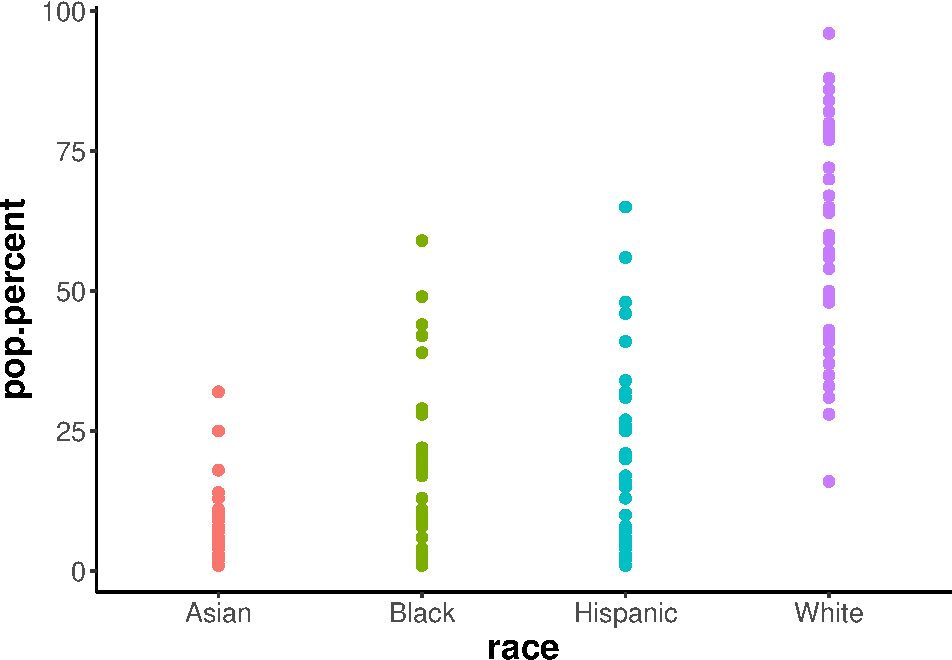
\includegraphics{ibad-ms_files/figure-latex/PLAY-race-plot-1.pdf}
\caption{}
\end{figure}

\begin{figure}
\centering
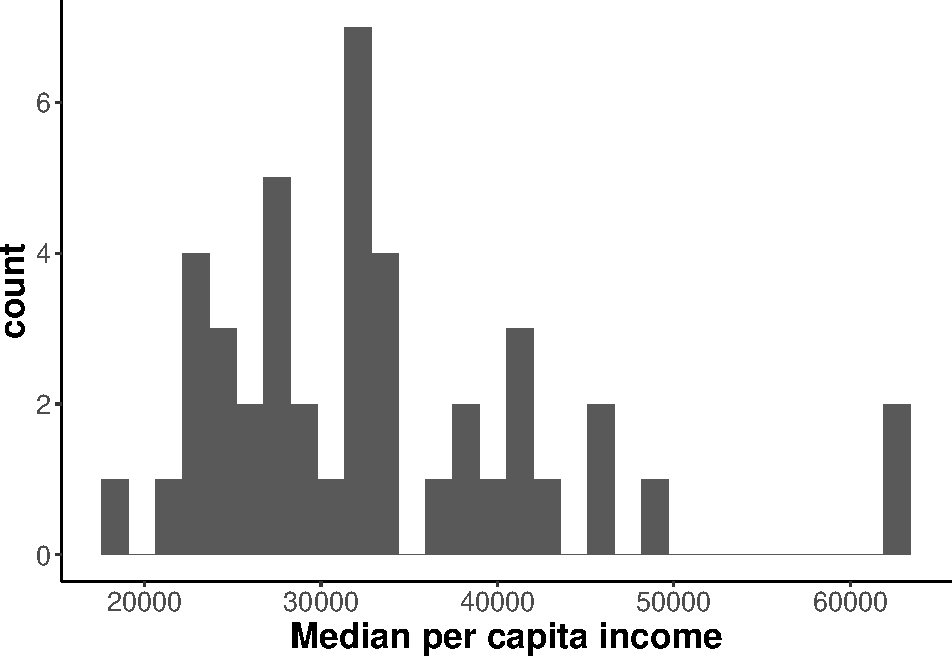
\includegraphics{ibad-ms_files/figure-latex/PLAY-econ-plot-1.pdf}
\caption{}
\end{figure}

We plan to collect data from \(n=900\) infant-mother dyads from 30
different communities located around the U.S. Each site will collect
data from 30 infants, 10 each at 12-, 18-, and 24-months of age (+/- 1
week), with equal numbers of females and males. Figure
\ref{fig:PLAY-sitemap} shows the proposed data collection sites and
non-collecting, data coding and analysis sites.

While not designed to be nationally representative, the data collection
sites are diverse in aggregate, based on Census data.
\ref{fig:PLAY-race-plot} shows the proportion of African American,
Hispanic/Latino, and Asian residents in the counties surrounding the
collection sites from which participating researchers will recruit.
Figure \ref{fig:PLAY-econ-plot} and figure \ref{fig:PLAY-ed-plot} show
economic and educational attainment indicators. Data collection sites
will have soft, advisory recruiting targets based on these sorts of
measures for their individual communities.

Readers may wish to know that these data are downloaded from the Census
Bureau using R's \texttt{choroplethr} \cite{choropletr} package.

\subsubsection{Material}\label{material-1}

\subsubsection{Procedure}\label{procedure-1}

\subsubsection{Data analysis}\label{data-analysis-1}

\section{General Discussion}\label{general-discussion}

\newpage

\section{References}\label{references}

\setlength{\parindent}{-0.5in} \setlength{\leftskip}{0.5in}

\hypertarget{refs}{}
\hypertarget{ref-R-papaja}{}
Aust, F., \& Barth, M. (2017). \emph{papaja: Create APA manuscripts with
R Markdown}. Retrieved from \url{https://github.com/crsh/papaja}

\hypertarget{ref-R-multilevel}{}
Bliese, P. (2016). \emph{Multilevel: Multilevel functions}. Retrieved
from \url{https://CRAN.R-project.org/package=multilevel}

\hypertarget{ref-R-googlesheets}{}
Bryan, J., \& Zhao, J. (2017). \emph{Googlesheets: Manage google
spreadsheets from r}. Retrieved from
\url{https://CRAN.R-project.org/package=googlesheets}

\hypertarget{ref-R-acs}{}
Glenn, E. H. (2018). \emph{Acs: Download, manipulate, and present
american community survey and decennial data from the us census}.
Retrieved from \url{https://CRAN.R-project.org/package=acs}

\hypertarget{ref-R-Hmisc}{}
Harrell Jr, F. E., Charles Dupont, \& others. (2017). \emph{Hmisc:
Harrell miscellaneous}.

\hypertarget{ref-R-purrr}{}
Henry, L., \& Wickham, H. (2017). \emph{Purrr: Functional programming
tools}. Retrieved from \url{https://CRAN.R-project.org/package=purrr}

\hypertarget{ref-R-choroplethrMaps}{}
Lamstein, A. (2017). \emph{ChoroplethrMaps: Contains maps used by the
'choroplethr' package}. Retrieved from
\url{https://CRAN.R-project.org/package=choroplethrMaps}

\hypertarget{ref-R-choroplethr}{}
Lamstein, A., \& Johnson, B. P. (2017). \emph{Choroplethr: Simplify the
creation of choropleth maps in r}. Retrieved from
\url{https://CRAN.R-project.org/package=choroplethr}

\hypertarget{ref-R-XML}{}
Lang, D. T., \& CRAN Team. (2018). \emph{XML: Tools for parsing and
generating xml within r and s-plus}. Retrieved from
\url{https://CRAN.R-project.org/package=XML}

\hypertarget{ref-R-bindrcpp}{}
Müller, K. (2016). \emph{Bindrcpp: An 'rcpp' interface to active
bindings}. Retrieved from
\url{https://CRAN.R-project.org/package=bindrcpp}

\hypertarget{ref-R-jsonlite}{}
Ooms, J. (2014). The jsonlite package: A practical and consistent
mapping between json data and r objects. \emph{arXiv:1403.2805
{[}Stat.CO{]}}. Retrieved from \url{https://arxiv.org/abs/1403.2805}

\hypertarget{ref-R-nlme}{}
Pinheiro, J., Bates, D., DebRoy, S., Sarkar, D., \& R Core Team. (2017).
\emph{nlme: Linear and nonlinear mixed effects models}. Retrieved from
\url{https://CRAN.R-project.org/package=nlme}

\hypertarget{ref-R-foreign}{}
R Core Team. (2017a). \emph{Foreign: Read data stored by 'minitab', 's',
'sas', 'spss', 'stata', 'systat', 'weka', 'dBase', ...} Retrieved from
\url{https://CRAN.R-project.org/package=foreign}

\hypertarget{ref-R-base}{}
R Core Team. (2017b). \emph{R: A language and environment for
statistical computing}. Vienna, Austria: R Foundation for Statistical
Computing. Retrieved from \url{https://www.R-project.org/}

\hypertarget{ref-R-psych}{}
Revelle, W. (2017). \emph{Psych: Procedures for psychological,
psychometric, and personality research}. Evanston, Illinois:
Northwestern University. Retrieved from
\url{https://CRAN.R-project.org/package=psych}

\hypertarget{ref-R-lattice}{}
Sarkar, D. (2008). \emph{Lattice: Multivariate data visualization with
r}. New York: Springer. Retrieved from
\url{http://lmdvr.r-forge.r-project.org}

\hypertarget{ref-R-survival-book}{}
Terry M. Therneau, \& Patricia M. Grambsch. (2000). \emph{Modeling
survival data: Extending the Cox model}. New York: Springer.

\hypertarget{ref-R-MASS}{}
Venables, W. N., \& Ripley, B. D. (2002). \emph{Modern applied
statistics with s} (Fourth.). New York: Springer. Retrieved from
\url{http://www.stats.ox.ac.uk/pub/MASS4}

\hypertarget{ref-R-gmodels}{}
Warnes, G. R., Bolker, B., Lumley, T., Randall C. Johnson are Copyright
SAIC-Frederick, R. C. J. C. from, Intramural Research Program, I. F. by
the, NIH, \ldots{} Cancer Research under NCI Contract NO1-CO-12400., C.
for. (2015). \emph{Gmodels: Various r programming tools for model
fitting}. Retrieved from
\url{https://CRAN.R-project.org/package=gmodels}

\hypertarget{ref-R-ggplot2}{}
Wickham, H. (2009). \emph{Ggplot2: Elegant graphics for data analysis}.
Springer-Verlag New York. Retrieved from \url{http://ggplot2.org}

\hypertarget{ref-R-plyr}{}
Wickham, H. (2011). The split-apply-combine strategy for data analysis.
\emph{Journal of Statistical Software}, \emph{40}(1), 1--29. Retrieved
from \url{http://www.jstatsoft.org/v40/i01/}

\hypertarget{ref-R-httr}{}
Wickham, H. (2017a). \emph{Httr: Tools for working with urls and http}.
Retrieved from \url{https://CRAN.R-project.org/package=httr}

\hypertarget{ref-R-tidyr}{}
Wickham, H. (2017b). \emph{Tidyr: Easily tidy data with 'spread()' and
'gather()' functions}. Retrieved from
\url{https://CRAN.R-project.org/package=tidyr}

\hypertarget{ref-R-tidyverse}{}
Wickham, H. (2017c). \emph{Tidyverse: Easily install and load
'tidyverse' packages}. Retrieved from
\url{https://CRAN.R-project.org/package=tidyverse}

\hypertarget{ref-R-forcats}{}
Wickham, H. (2018a). \emph{Forcats: Tools for working with categorical
variables (factors)}. Retrieved from
\url{https://CRAN.R-project.org/package=forcats}

\hypertarget{ref-R-stringr}{}
Wickham, H. (2018b). \emph{Stringr: Simple, consistent wrappers for
common string operations}. Retrieved from
\url{https://CRAN.R-project.org/package=stringr}

\hypertarget{ref-R-dplyr}{}
Wickham, H., \& Francois, R. (2016). \emph{Dplyr: A grammar of data
manipulation}. Retrieved from
\url{https://CRAN.R-project.org/package=dplyr}

\hypertarget{ref-R-tibble}{}
Wickham, H., Francois, R., \& Müller, K. (2017). \emph{Tibble: Simple
data frames}. Retrieved from
\url{https://CRAN.R-project.org/package=tibble}

\hypertarget{ref-R-readr}{}
Wickham, H., Hester, J., \& Francois, R. (2017). \emph{Readr: Read
rectangular text data}. Retrieved from
\url{https://CRAN.R-project.org/package=readr}

\hypertarget{ref-R-Formula}{}
Zeileis, A., \& Croissant, Y. (2010). Extended model formulas in R:
Multiple parts and multiple responses. \emph{Journal of Statistical
Software}, \emph{34}(1), 1--13. Retrieved from
\url{http://www.jstatsoft.org/v34/i01/}






\end{document}
